% BEGIN PREAMBEL
\documentclass[9pt, xcolor=dvipsnames]{beamer}
\usepackage[british]{babel}
\usepackage{multimedia}
\usepackage{amsmath,amsfonts,amssymb}
\usepackage{upgreek}
\usepackage{pgfpages}
\usepackage[version=4]{mhchem}
\usepackage{chemformula}
\usepackage{lmodern}
\usepackage{graphicx}
\usepackage{multicol}
\usepackage{multirow}
\usepackage{color}
\usepackage{xcolor,fontawesome}
\usepackage{wrapfig}
\usepackage{siunitx}
\sisetup{detect-weight=true, detect-family=true}
\usepackage{fontspec}
\usepackage{tikz}
\usepackage{textpos}
\usepackage{booktabs}
\usepackage{caption}
\usepackage{subcaption}
\usepackage{wasysym}
\usepackage{animate}
\usepackage{tabularx}
\usepackage{ETHlogo}
\usepackage{xfrac}
\usepackage{tikz-feynman}
\newfontfamily\ubuntu{Ubuntu}
\newcommand{\as}{\\[14pt]}
\newcommand{\s}{\\[7pt]}
\newcommand{\is}{\\[2pt]}
\newcommand{\no}{\noindent}
\newcommand{\ka}{\hspace*{0.5cm}}
\newcommand{\ma}{\hspace*{1cm}}
\newcommand{\ga}{\hspace*{1.5cm}}
\newcommand{\li}{\left|}
\newcommand{\re}{\right|}
\newcommand{\const}{\text{const.}}
\newcommand{\z}{\text}
\newcommand{\terminal}[1]{\colorbox{black}{\textcolor{white}{{\fontfamily{phv}\selectfont \scriptsize{#1}}}}}
\newcommand{\plugin}[1]{\textit{\flq#1\frq}}
\newcommand{\ra}{$\rightarrow$ }
\definecolor{cadmiumgreen}{rgb}{0.0, 0.42, 0.24}
\newcommand{\itemfill}{\setlength{\itemsep}{\fill}}
\newcommand{\orderof}[1]{$\mathcal{O}\left(#1\right)$}
\newcommand{\fig}[2]{\begin{figure}\centering\includegraphics[height={#2}\textheight]{#1}\end{figure}}
\newcommand{\figc}[3]{\begin{figure}\centering\includegraphics[height={#2}\textheight]{#1}\caption{#3}\end{figure}}
\newcommand{\figp}[2]{\begin{figure}\centering\includegraphics[width={#2}\textheight, angle=-90]{#1}\end{figure}}
\newcommand{\subfig}[4][0.45]{\begin{subfigure}{{#1}\textwidth}\centering
			\includegraphics[height={#3}\textheight]{#2}
			\caption{#4}\end{subfigure}}
\newcommand{\subfigp}[3]{\begin{subfigure}{0.45\textwidth}\centering
			\includegraphics[width={#2}\textheight, angle=-90]{#1}
			\caption{#3}\end{subfigure}}

\usetheme{Boadilla}
\graphicspath{ {Pics/} }
\makeatletter
\def\input@path{ {sections/} }
\makeatother
\usecolortheme[named=ForestGreen]{structure}
\useoutertheme{miniframes}
\beamertemplatenavigationsymbolsempty
\makeindex
\author[M. Reichmann]{Michael Reichmann}
\institute[\textbf{\textit{ETH}}\scalebox{.6}{\textit{Z\"{u}rich}}]{Swiss Federal Institute of Technology Zurich}
\AtBeginSection{\frame[noframenumbering]{\sectionpage}}

\setbeamercolor{frametitle}{bg=date in head/foot.bg!20!white}

%% TITLE PAGE
\defbeamertemplate*{title page}{customized}[1][] {
	\ETHlogo[3cm]
	\vspace*{-33pt}
	\begin{figure}[t]
		\flushright
		
\includegraphics[height=2.0cm]{IPA.png}
	\end{figure}
	\vspace*{-10pt}
	\begin{figure}
		\centering
		
\includegraphics[width=.26\textheight]{T.png}
		\hspace{6cm}
		
\includegraphics[width=.35\textheight]{B.png}
	\end{figure}
	\vspace*{-10pt}
	\begin{block}{}
		\centering
		\vspace*{1pt}
		\usebeamerfont{title}\usebeamercolor[fg]{title}\textbf{\inserttitle}\\\vspace*{5pt}
		\usebeamerfont{subtitle}\insertsubtitle\\\vspace*{1pt}
	\end{block}
	\vspace*{10pt}
	\centering
	\color{black}
	\usebeamerfont{author}\textbf{\insertauthor}\par\vspace*{5pt}
	\usebeamerfont{date}\insertdate\par
}

%% FOOTLINE
\setbeamertemplate{footline}
{
  \leavevmode%
  \hbox{%
  \begin{beamercolorbox}[wd=.3\paperwidth,ht=2.25ex,dp=1ex,center]{author in head/foot}%
    \usebeamerfont{author in head/foot}\insertshortauthor\hspace*{2pt}
    (
\includegraphics[height=3.5pt]{ETHLogoWhite})
  \end{beamercolorbox}%
  \begin{beamercolorbox}[wd=.4\paperwidth,ht=2.25ex,dp=1ex,center]{title in head/foot}%
    \usebeamerfont{title in head/foot}\insertshorttitle
  \end{beamercolorbox}%
  \begin{beamercolorbox}[wd=.3\paperwidth,ht=2.25ex,dp=1ex,right]{date in head/foot}%
    \usebeamerfont{date in head/foot}\insertdate\hspace*{3em}
    \insertframenumber{} / \inserttotalframenumber\hspace*{1ex}
  \end{beamercolorbox}}%
  \vskip0pt%
}
 
%% SECTION PAGE
\setbeamertemplate{section page}
{
    \begin{centering}
		\usebeamerfont{title}Section \insertsectionnumber\\\vspace*{.7cm}
		\begin{beamerboxesrounded}[shadow=true, lower=frametitle]{}
			\centering
			\vspace*{3pt}
			\usebeamerfont{frametitle}\textbf{\insertsection}\par
			\vspace*{3pt}
		\end{beamerboxesrounded}
    \end{centering}
}

\title[Heavy Quarks]{The Discovery of the Heavy Quarks}
\subtitle{Experimental Foundations of Particle Physics}
% END PREAMBEL

\begin{document}

% ============= TITLE PAGE =============
\usebackgroundtemplate{\tikz\node[opacity=0.2] {\hspace*{-5pt}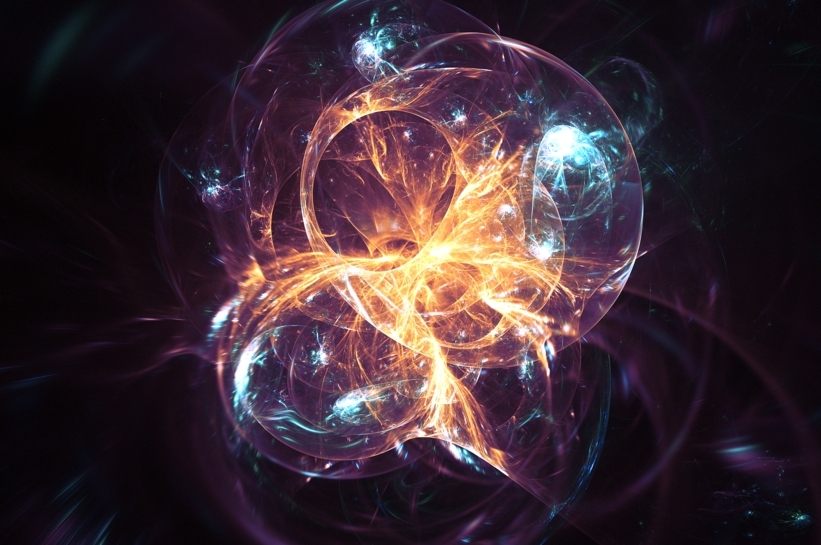
\includegraphics[height=\paperheight,width=1.05\paperwidth]{back.jpg}};}
\maketitle
\usebackgroundtemplate{}

% ============= TABLE OF CONTENTS ======
\begin{frame}%[allowframebreaks]
	\frametitle{Table of contents}
	\tableofcontents[hideallsubsections]   % [pausesections]
\end{frame}

% ============= 1 =============
\section{Introduction}
\begin{frame}{Introduction}
	
	\begin{minipage}[c][.7\textheight]{.6\textwidth}
		\begin{itemize}
			\itemfill
			\item<1-> in 1974 (with J/$\uppsi$) 4 leptons and 4 quarks discovered
			\item<2-> in 1975 Perl et al. discovered $\uptau$-lepton and its neutrino
			\item<2-> in 1973 6-plet proposed by Kobayashi and Maskawa to describe CP violation
			\item<2-> indiction of another pair of quarks
			\item<3-> in 1977 discovery of the bottom (beauty) quark 
			\item<3-> postulation of a sixth quark
			\item<4-> in 1995 discovery of the top (truth) quark
			\item<4-> complete set of fermions until now
		\end{itemize}
	\end{minipage}
	\hfill
	\begin{minipage}{.37\textwidth}
		\only<1>{\fig{sm2}{.8}}
		\only<2>{\fig{sm1}{.8}}
		\only<3>{\fig{sm3}{.8}}
		\only<4>{\fig{sm}{.8}}
	\end{minipage}


\end{frame}


% ============= 2 =============
\section{The Beauty Quark}
\begin{frame}{The $\Upupsilon$-Meson}
 
	\begin{minipage}[c][.2\textheight]{.8\textwidth}
	 	\begin{itemize}
			\item bound state of \textbf{b$\bar{\z{b}}$}\vspace*{10pt}
			\item decay channels:
		\end{itemize}
	\end{minipage}
	\begin{minipage}{.18\textwidth}
		\fig{T1}{.2}
	\end{minipage}
	
	\begin{figure}
		\subfig[.37]{diag2}{.25}{\SI{82}{\%}}
		\subfig[.26]{diag1}{.25}{\SI{9}{\%}}
		\subfig[.35]{diag3}{.25}{\SI{2}{\%}}
	\end{figure}
	\begin{itemize}\itemfill
		\item mostly decay into gluons which hadronise \ra signals mostly caused by hadrons
		\item leptonic decay splits up into \SIrange{2.5}{3}{\%} for each e, $\upmu$ and $\uptau$
	\end{itemize}

\end{frame}

%%%%%%%%%%%%%%%%%%%%%%%% FRAME 1 %%%%%%%%%%%%%%%%%%%%%%%%%%%%%%%
\subsection{Discovery}
\begin{frame}{Discovery Paper}

	\fig{BDis}{.84}
	
\end{frame}

%%%%%%%%%%%%%%%%%%%%%%%% FRAME 2 %%%%%%%%%%%%%%%%%%%%%%%%%%%%%%%
\begin{frame}{Setup}
 
	\vspace*{-10pt}
	\only<1>{\fig{BSetup}{.72}}
	\only<2>{\fig{BSetup1}{.72}}
	\only<3>{\fig{BSetup2}{.72}}
	\only<4>{\fig{BSetup3}{.72}}
	\only<5>{\fig{BSetup4}{.72}}
	\only<6>{\fig{BSetup5}{.72}}
	\only<7>{\fig{BSetup6}{.72}}
	\only<8>{\fig{BSetup7}{.72}}
	\only<9>{\fig{BSetup8}{.72}}
	\only<10>{\fig{BSetup9}{.72}}
	
	\begin{minipage}[c][.15\textheight]{\textwidth}
		\begin{itemize}
			\only<1>{\item[] } 
			\only<2>{\item \SI{400}{\giga\electronvolt} proton beam shot on narrow target (Pt/Cu) with \SI{30}{\%} interaction length} 
			\only<3>{\item hadron filter out of Be with 18 interaction length (\SIrange{3}{5}{^{\circ}} horiz. and \SI{\pm.5}{^{\circ}} vert.)}
			\only<4>{\item heavy metal (Steel, W) shielding to minimise particle leakage}
			\only<5>{\item tungsten beam dump} 
			\only<6>{\item additional shielding out of polyethylene and more steel}
			\only<7>{\item spectrometer dipole magnets with horizontal field}
			\only<7>{\item both arms are symmetric to drawing plane and detect $\upmu^{+}$ and $\upmu^{-}$}
			\only<8>{\item scintillation hodometers and wire chambers for tracking (limit of \SI{10e7}{counts\per s})}
			\only<9>{\item solid iron magnet to partially refocus and redetermine muon momentum}
			\only<10>{\item \v{C}erenkov counter to prevent low momentum muon triggers}
		\end{itemize}
	\end{minipage}

\end{frame}
%%%%%%%%%%%%%%%%%%%%%%%% FRAME 3 %%%%%%%%%%%%%%%%%%%%%%%%%%%%%%%
\begin{frame}{Intermezzo: Sideband Fit}
 
	\vspace*{-10pt}
	\only<1>{\hspace*{-20pt}\figp{SB1}{.60}}
	\only<2>{\hspace*{-20pt}\figp{SB2}{.60}}
	\only<3>{\hspace*{-20pt}\figp{SB3}{.60}}
	\only<4>{\hspace*{-20pt}\figp{SB4}{.60}}
	\only<5>{\hspace*{-20pt}\figp{SB5}{.60}}
	\only<6>{\hspace*{-20pt}\figp{SB6}{.60}}
	
	\begin{minipage}[c][.15\textheight]{\textwidth}
		\begin{itemize}
			\only<1>{\item typical shape of data in particle physics: continuous background with a small bump} 
			\only<2>{\item background extraction with a fit of the whole set does not work well} 
			\only<3>{\item divide the data set in a signal and two background parts (\ra side bands)}
			\only<4>{\item fitting just the side bands yields a much better result}
			\only<5>{\item getting the signal distribution by subtracting the full data set by the fit} 
			\only<6>{\item get width and position of the signal by a fit}
		\end{itemize}
	\end{minipage}

\end{frame}
%%%%%%%%%%%%%%%%%%%%%%%% FRAME 4 %%%%%%%%%%%%%%%%%%%%%%%%%%%%%%%
\begin{frame}{Results}
 
	\begin{minipage}[c][.8\textheight]{.78\textwidth}
		\begin{itemize}
			\itemfill
			\item statistically significant enhancement at \SI{9.5}{\giga\electronvolt} $\upmu^{+}\upmu^{-}$ mass
			\item solid line background fit using side band method
			\begin{equation*} \dfrac{\z{d}^2\upsigma}{\z{dmdy}} = \z{A}\mathrm{e}^{-\z{bm}} \end{equation*}
			\item fit expects 350 events in excluded region but 770 events in data
			\item bump wider than resolution of detector (FWHM: \SI{.5\pm.1}{\giga\electronvolt})
			\item simple Gaussian fit of background subtracted data yields:
			{\usebeamercolor[fg]{title}\begin{align*}
				\z{\textbf{m}} &= \textbf{\SI{9.54\pm.04}{\giga\electronvolt}}\\
				\z{\textbf{FWHM}} &= \textbf{\SI{1.16\pm.09}{\giga\electronvolt}}
			\end{align*}}
			\item same goodness of fit with two Gaussians with fixed with of detector resolution \ra later $\Upupsilon$ and $\Upupsilon'$

		\end{itemize}

	\end{minipage}
	\begin{minipage}{.2\textwidth}
		\figc{BRes1}{.69}{\scriptsize{dimuon production cross section as a function of invariant mass}}
	\end{minipage}

	
\end{frame}

%%%%%%%%%%%%%%%%%%%%%%%% FRAME 5 %%%%%%%%%%%%%%%%%%%%%%%%%%%%%%%
\begin{frame}{Verification}

	\begin{itemize}\itemfill
		\item same sign dimuon spectrum ($\upmu^{+}\upmu^{+}$ and $\upmu^{-}\upmu^{-}$)
		\begin{itemize}
			\item upper limit on combined effects of accidental coincidences and hadronic decays
		\end{itemize}
		\item re-measurement of the muon momentum by the second magnet and by PCW at the centre of the first magnet
		\begin{itemize}
			\item avoid misidentified \ch{\ensuremath{\uppsi}->\ensuremath{\upmu^+}+\ensuremath{\upmu^-}} at high mass
			\item confirmed by clear separation of the $\uppsi$ and $\uppsi'$ in the Figure
		\end{itemize}
	\end{itemize}
	
	\begin{minipage}[c][.35\textheight]{0.58\textwidth}
		\begin{itemize}\itemfill
			\item study of various subsets of the data with different magnetic fields
			\begin{itemize}
				\item check for apparatus bias
			\end{itemize}
			\item study of data with and without target
			\begin{itemize}
				\item rule out signal created from beam dump
			\end{itemize}
		\end{itemize}
	\end{minipage}
	\begin{minipage}{.4\textwidth}
		\fig{BRes}{.4}
	\end{minipage}\vspace*{-20pt}

	
\end{frame}

%%%%%%%%%%%%%%%%%%%%%%%% FRAME 6 %%%%%%%%%%%%%%%%%%%%%%%%%%%%%%%
\subsection{Further Experiments}
\begin{frame}{PLUTO Collaboration Paper}

	\fig{BPluto}{.84}
	
\end{frame}

%%%%%%%%%%%%%%%%%%%%%%%% FRAME 7 %%%%%%%%%%%%%%%%%%%%%%%%%%%%%%%
\begin{frame}{PLUTO Detector}
 
	\vspace*{-10pt}
	\only<1>{\fig{PlutoDet}{.72}}
	\only<2>{\fig{PlutoDet5}{.72}}
	\only<3>{\fig{PlutoDet1}{.72}}
	\only<4>{\fig{PlutoDet2}{.72}}
	\only<5>{\fig{PlutoDet3}{.72}}
	\only<6>{\fig{PlutoDet4}{.72}}
	
	\begin{minipage}[c][.15\textheight]{\textwidth}
		\begin{itemize}
			\only<1>{\item[]  } 
			\only<2>{\item up to \SI{5}{\giga\electronvolt} electron beams collided in the centre} 
			\only<3>{\item cylindrical proportional wire chamber with \SI{92}{\%} coverage}
			\only<3>{\item tracking and momentum measurement}
			\only<4>{\item cylindrical array of shower counters with \SI{8.6}{radiation length} and \SI{94}{\%} coverage}
			\only<4>{\item calorimeter to measure the full energy}
			\only<5>{\item magnet with \SI{1.69}{\tesla}}
			\only<6>{\item muon chambers}
		\end{itemize}
	\end{minipage}

\end{frame}
%%%%%%%%%%%%%%%%%%%%%%%% FRAME 8 %%%%%%%%%%%%%%%%%%%%%%%%%%%%%%%
\begin{frame}{Results}
	
	\begin{minipage}[c][.4\textheight]{0.65\textwidth}
		\begin{itemize}\itemfill
			\item acquiring cross section by scanning $\sqrt{s}$ in steps of either \SI{5}{\giga\electronvolt} or \SI{10}{\giga\electronvolt}
			\item only considering hadronic decay products
			\item remove 1/s background
			\item reduce cosmic ray background by use of bunch crossing time (bunched beam structure vs continuous background)
		\end{itemize}
	\end{minipage}
	\begin{minipage}{.31\textwidth}
		\figc{BPlutoRes}{.3}{\footnotesize{total cross section for hadron production}}
	\end{minipage}
	
	\begin{itemize}\itemfill
		\item remove QED events with coplanarity cut and shower recognition
		\item remove beam gas interaction by cuts on visible energy and missing mass
		\item fitting data with Gaussian yields:
		{\usebeamercolor[fg]{title}\begin{align*}
			\z{\textbf{m}} &= \textbf{\SI{9.46\pm.01}{\giga\electronvolt}}\\
			\mathbf{\upsigma_{\z{Gauss}}} &= \textbf{\SI{7.8\pm.9}{\mega\electronvolt}}
		\end{align*}}
	\end{itemize}\vspace*{-20pt}

	
\end{frame}
%%%%%%%%%%%%%%%%%%%%%%%% FRAME 9 %%%%%%%%%%%%%%%%%%%%%%%%%%%%%%%
\begin{frame}{Charge}
	
	\begin{itemize}\itemfill
		\item relation of total hadronic cross section to resonance mass and the resonance width
		\begin{equation*} \int\upsigma_{\z{h}}\z{dM} = \frac{6\uppi^{2}}{{\z{M}_{\z{R}}}^{2}}\frac{\Upgamma_{\z{ee}}\Upgamma_{\z{h}}}{\Upgamma_{\z{tot}}} \end{equation*}
		\item standard assumption: $\Upgamma_{\z{tot}}\approx\Upgamma_{\z{h}}$ \ra direct measurement of $\Upgamma_{\z{ee}}$
		{\usebeamercolor[fg]{title}\begin{equation*} \Upgamma_{\z{ee}} = \SI{1.3\pm.4}{\kilo\electronvolt} \end{equation*}}\vspace*{-20pt}
		\item theoretical predictions from the same model:
		\begin{center}
			\begin{tabular}{c|c|c}
						\multirow{2}{*}{Decay Mode}	& \multicolumn{2}{c}{Width [\SI{}{\kilo\electronvolt}]}\\\cline{2-3}
													& $\z{e} = \pm\sfrac{1}{3}$	& $\z{e} = \pm\sfrac{2}{3}$\\\hline
						$\upmu^{+}\upmu^{-}$ 		& \SI{.70\pm.09}{} 	& \SI{2.8\pm.4}{}
			\end{tabular}		             
		\end{center}\vspace*{10pt}
		\item \usebeamercolor[fg]{title}\textbf{implies charge of -\sfrac{1}{3} for the bottom quark}

	\end{itemize}

	
\end{frame}

% ============= 3 =============
\section{The Truth Quark}
\begin{frame}{Introduction}

	\begin{minipage}[c][.23\textheight]{.8\textwidth}
		\begin{itemize}
			\itemfill
			\item in early 90s all SM particles except H and t-quark discovered
			\item beauty discovery \ra weak isospin partner was undoubted
			\item quark masses are fundamental parameters in the SM
		\end{itemize}
	\end{minipage}
	\begin{minipage}{.18\textwidth}
		\fig{B1}{.2}
	\end{minipage}
	
	\begin{itemize}\itemfill
		\item early estimates: $\z{m}_{\z{t}} \approx 3 \z{m}_{\z{b}} \approx \SI{15}{\giga\electronvolt}$
		\item many new accelerator could only push limits higher:
		\item TRISTAN ($e^+e^-$) at KEK (Tsukuba, Japan) with $\sqrt{s} = \SI{61.4}{\giga\electronvolt}$ \ra \SI{30.2}{\giga\electronvolt}
		\item Sp$\overline{\z{p}}$S at CERN with $\sqrt{s} = \SI{630}{\giga\electronvolt}$ \ra \SI{69}{\giga\electronvolt}
		\item SLC ($e^+e^-$) at Stanford and LEP ($e^+e^-$) at CERN \ra $\sfrac{1}{2} \z{m}_{\z{t}}$
		\item hadron collider needed (\ra Tevatron)
	\end{itemize}
	
\end{frame}
%%%%%%%%%%%%%%%%%%%%%%%% FRAME 1 %%%%%%%%%%%%%%%%%%%%%%%%%%%%%%%
\begin{frame}{Decay Channels (1)}

	\begin{itemize}\itemfill
		\item estimate on $\z{m}_{\z{t}}$ in 1994: \SI{\sim180}{\giga\electronvolt}
		\item prior to discovery: behaviour completely predicted by SM
		\item $\z{m}_{\z{t}} > \z{m}_{\z{W}}$ \ra main decay channel (\SI{\sim95}{\%}):\ka{\usebeamercolor[fg]{title}\textbf{t\ch{->}$\z{W}^+\z{b}$}}
		\begin{equation*} \Upgamma_{\z{t}} = \frac{\z{G}_{\z{F}}\z{m}_{\z{t}}^{3}}{8\uppi\sqrt{2}}\left(1 - \frac{\z{m}_{\z{W}}^{2}}{\z{m}_{\z{t}}^{2}}\right)^{2}\left(1 + 2\frac{\z{m}_{\z{W}}^{2}}{\z{m}_{\z{t}}^{2}}\right)\end{equation*}
		\item width for the expected mass: \SI{\sim1}{\giga\electronvolt} \ra decay before hadronisation
	\end{itemize}
	
	\begin{figure}\vspace*{-10pt}
		\centering
		\subfig[.3]{tWbq}{.25}{\SI{\sim60}{\%}}
		\subfig[.3]{tWbl}{.25}{\SI{\sim40}{\%}}
	\end{figure}\vspace*{-10pt}
	
	\begin{itemize}\itemfill
		\item leptonic decay equally splits up into $e$, $\upmu$ and $\uptau$
	\end{itemize}

\end{frame}
%%%%%%%%%%%%%%%%%%%%%%%% FRAME 2 %%%%%%%%%%%%%%%%%%%%%%%%%%%%%%%
\begin{frame}{Decay Channels (2)}

	\begin{itemize}\itemfill
		\item top mostly pair produced via $\z{q}\overline{\z{q}}$\ch{->}$\z{t}\overline{\z{t}}$ or gluon fusion: $\z{g}\z{g}$\ch{->}$\z{t}\overline{\z{t}}$  
		\item main decay of the top pair: $\z{t}\overline{\z{t}}$\ch{->}$\z{W}^+\z{b}\z{W}^-\overline{\z{b}}$
		\item b decay:
	\end{itemize}
	
	\begin{figure}\vspace*{-10pt}
		\centering
		\subfiga[.3]{BDec2}{.25}\hspace*{10pt}
		\subfiga[.4]{BDec1}{.25}
	\end{figure}
	
	\begin{itemize}\itemfill
		\item typical signals:
		\begin{itemize}
			\item 2 b-jets + dilepton ($e^+e^-$, $\upmu^+\upmu^-$, $e^+\upmu^-$, $\upmu^+e^-$)
			\item 2 b-jets + single lepton + two jets
			\item 2 b-jets + 4 jets
		\end{itemize}
		\item huge background on pure QCD process due to other more common QCD processes
		\item how to discriminate b-jets from other jets?
	\end{itemize}

\end{frame}
%%%%%%%%%%%%%%%%%%%%%%%% FRAME 3 %%%%%%%%%%%%%%%%%%%%%%%%%%%%%%%
\begin{frame}{B-Tagging}

	\begin{itemize}\itemfill
		\item how to discriminate b-jets from other jets?
	\end{itemize}

\end{frame}
%%%%%%%%%%%%%%%%%%%%%%%% FRAME 4 %%%%%%%%%%%%%%%%%%%%%%%%%%%%%%%
\begin{frame}{$\z{t}\overline{\z{t}}$ Cross Section}

	\vspace*{-10pt}\fig{ttcs}{.65}\vspace*{-10pt}
	
	\begin{itemize}\itemfill
		\item cross section extracted from SM
		\item Tevatron Lumi in 1995: \SI{10e30}{\per\centi\meter\squared\per\second}
		\begin{equation*} \z{R}_{\z{t}\overline{\z{t}}} = \upsigma_{\z{t}\overline{\z{t}}}\mathscr{L} = \SI{.1}{\hertz}\end{equation*}

	\end{itemize}

\end{frame}
\subsection{Discovery at CDF}
%%%%%%%%%%%%%%%%%%%%%%%% FRAME 5 %%%%%%%%%%%%%%%%%%%%%%%%%%%%%%%
\begin{frame}{Discovery Paper (1)}
	\fig{TDis1}{.84}
\end{frame}
%%%%%%%%%%%%%%%%%%%%%%%% FRAME 6 %%%%%%%%%%%%%%%%%%%%%%%%%%%%%%%
\begin{frame}{Discovery Paper (2)}
	\fig{TDis2}{.84}
\end{frame}
%%%%%%%%%%%%%%%%%%%%%%%% FRAME 7 %%%%%%%%%%%%%%%%%%%%%%%%%%%%%%%
\begin{frame}{CDF Detector (1)}[plain]
	\begin{tikzpicture}[remember picture,overlay]
		\node[at=(current page.center)] {
			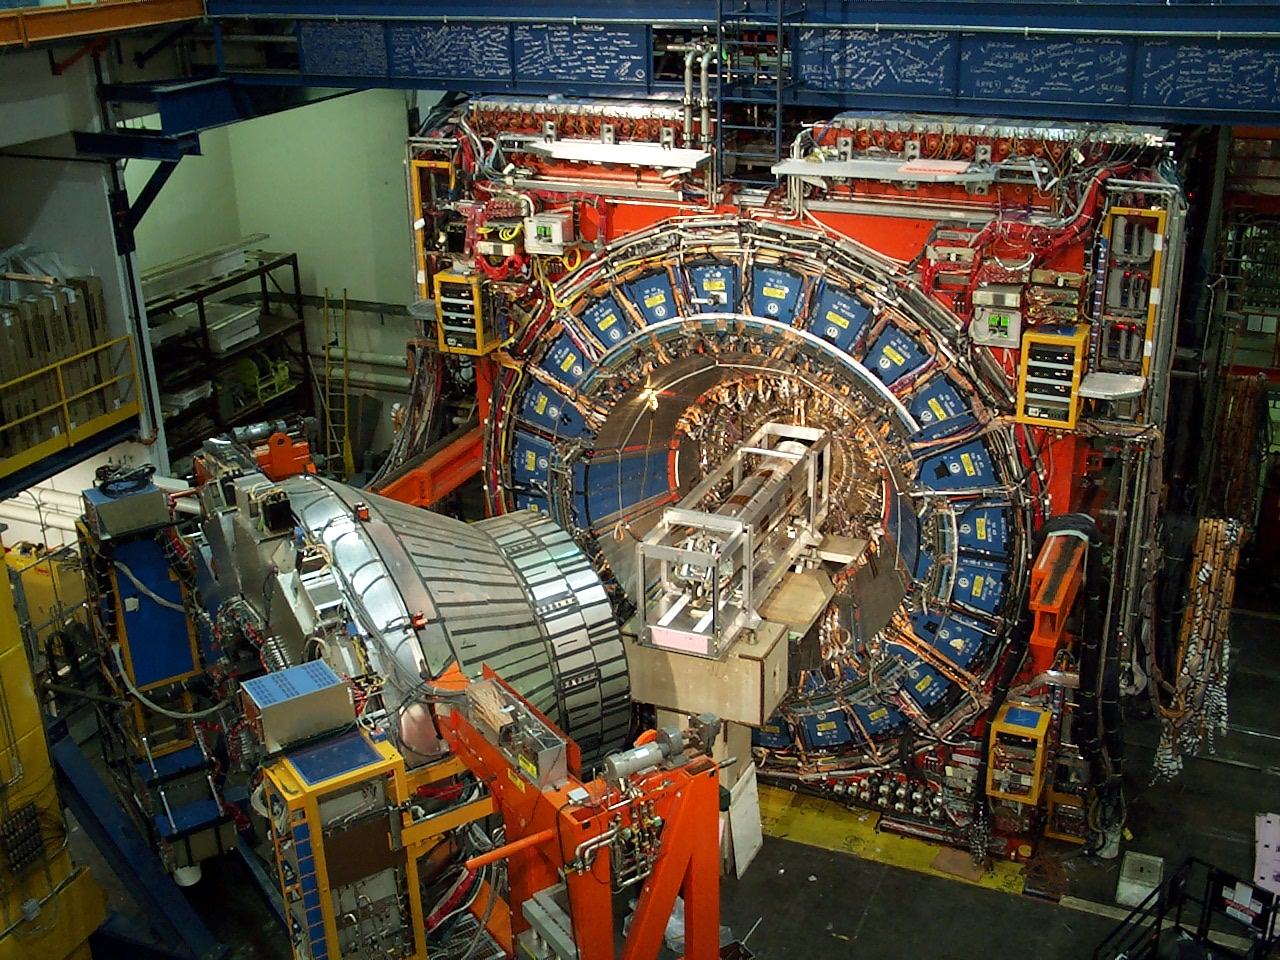
\includegraphics[width=\paperwidth]{cdfdet}
		};
	\end{tikzpicture}
\end{frame}
%%%%%%%%%%%%%%%%%%%%%%%% FRAME 8 %%%%%%%%%%%%%%%%%%%%%%%%%%%%%%%
\begin{frame}{CDF Detector}
	\fig{CDFDet1}{.84}
\end{frame}
%%%%%%%%%%%%%%%%%%%%%%%% FRAME 9 %%%%%%%%%%%%%%%%%%%%%%%%%%%%%%%
\begin{frame}{Introduction}
	
	\begin{itemize}\itemfill
		\item paper from 1994 with estimate on mass and cross section
		\item using dataset of \SI{19}{\per\pico\barn} + \SI{47}{\per\pico\barn} (\ra $\sim$ 400 events)
		\item looking at two decay channels
		\begin{itemize}
			\item dilepton
			\item lepton + jets
		\end{itemize}
		\item both data samples subsets of events with isolated leptons with high $P_{T}>\SI{20}{\giga\electronvolt}$
		\item cut on invariant mass of dilepton $\SI{75}{\giga\electronvolt}<\z{m}_{\z{I}}<\SI{105}{\giga\electronvolt}$ \ra exclude Z events
		\item main background reduction by b-tagging
		\begin{itemize}
			\item reconstruction of secondary vertices from b decay in SVX \ra SVX tag 
			\item finding additional leptons from b decay in ECAL \ra SLT tag 
		\end{itemize}
	\end{itemize}

\end{frame}
%%%%%%%%%%%%%%%%%%%%%%%% FRAME 10 %%%%%%%%%%%%%%%%%%%%%%%%%%%%%%%
\begin{frame}{Lepton + Jets Channel}
	
	\underline{\textbf{SVX tagging:}}\vspace*{5pt}
	\begin{itemize}\itemfill 
		\item search for secondary vertices with three ore more tracks
		\item then search for two ore more tracks with more stringed track and vertex quality
		\item efficiency estimated by $e$, $\upmu$ samples with enriched b decays (\SI{96}{\%} agreement to MC)
		\item tagging efficiency: \SI{42\pm5}{\%}
	\end{itemize}
	
	\begin{minipage}[c][.30\textheight]{.64\textwidth}
	 	\begin{itemize}\itemfill
			\item backgrounds from recoil of heavy quark pairs against W and mistags
	 	 	\item for $\z{W}+\ge3$ jets: observation of \SI{27}{tags} with bg of \SI{6.7\pm2.1}{tags}
	 	 	\item decay lifetime of SVX tags agrees well with MC
	 	\end{itemize}
	\end{minipage}
	\begin{minipage}{.33\textwidth}
		\fig{CDFRes1}{.45}
	\end{minipage}

\end{frame}
%%%%%%%%%%%%%%%%%%%%%%%% FRAME 11 %%%%%%%%%%%%%%%%%%%%%%%%%%%%%%%
\begin{frame}{Dilepton Channel}
	
	\begin{minipage}[c][.30\textheight]{.64\textwidth}
		\begin{itemize}\itemfill 
			\item major backgrounds:
			\begin{itemize}
				\item Drall-Yan process
				\item Z\ch{->}$\uptau\uptau$
				\item misidentified hadrons
				\item WW, b$\overline{\z{b}}$
			\end{itemize}
		\end{itemize}
	\end{minipage}
	\begin{minipage}{.33\textwidth}
		\fig{DrellYan}{.3}
	\end{minipage}

\end{frame}



% ============= CONCLUSION =============
\section{Conclusion}
\begin{frame}{Conclusion}
	\begin{minipage}[c][4cm]{\textwidth}
		\begin{itemize}
			\itemfill
			\item empty
			\item moreempty
			\item moremoreempty
		\end{itemize}
	\end{minipage}
\end{frame}


% DOCUMENT END
\end{document}

